\documentclass{article}
\usepackage{graphicx}
\usepackage{float}
\usepackage{mhchem}
\usepackage{physics}
\usepackage{amsfonts}
\usepackage{natbib}
  % or plainnat, abbrvnat

\title{Investigating Topological Phase Transitions in three-dimensional Quantum Spin Liquids with Neural Quantum States}
\author{SURF Proposal}
\date{Sanzhar Bissenali\\
Harvard University\\
Mentors: Prof. Norman Yao and Dr. Sajant Anand \\
Associate Mentor: Prof. Marco Bernardi
}

\begin{document}
\maketitle

\section{Introduction}
Quantum information is a rapidly evolving field with the potential to revolutionize computing, communication, and sensing technologies. In principle, by leveraging inherently quantum-mechanical phenomena such as superposition and entanglement, the field promises breakthroughs that are unreachable in a "classical" way [1]. However, addressing real-world problems in quantum information requires overcoming several key challenges, including quantum decoherence, scalability, and the development of efficient quantum algorithms and hardware.

One of the current areas of active research in quantum computation is the design of coherent, scalable, and noise-resistant quantum hardware. The direction pursued by big tech companies such as Google and IBM is related to superconducting qubits [2]. Their inherent advantage lies in high-speed gates (nanosecond scale), high scalability due to fabrication methods developed in the semiconductor industry, and their natural suitability to implement the Surface Code, the prototypical two-dimensional topological quantum error-correction code, first introduced by Alexei Kitaev in 1997 [3,4]. 

Although two-dimensional surface codes have high-error thresholds and have been experimentally verified, they require many rounds of error correction and can be costly to implement a universal fault-tolerant quantum computer [5]. On the other hand, with the configurable architecture devices, such as 3D-optical tweezer arrays and trapped ion simulators, we can go beyond 2D. Naturally, we can consider the 3D surface code as an extension of the 2D version on the cubic lattice. It has been shown that this type of surface code allows a single-shot error correction and transversal non-Clifford gates, which simplifies the implementation of a universal fault-tolerant quantum computer [6]. 

\pagebreak

However, the properties of the 3D surface code are much less understood compared to the 2D variant, particularly its robustness to external magnetic field perturbations and deformations. \textbf{In this work, we want to investigate the topological order and ground state stability of the 3D surface code to magnetic field perturbations.}

The 2D Surface code, defined on a square lattice, is described by a Hamiltonian given by the equation (1)
\begin{equation}
    H = - \sum_v A_v - \sum_p B_p  
\end{equation}
where $A_v, B_p$ are 4-body stabilizers around a vertex and plaquette, respectively. The ground state of this Hamiltonian has an emergent phenomena  of $\mathbb{Z}_2$ spin liquid. This is precisely the reason why they have attracted significant attention from both theoretical and computational perspectives. Proven, long-established tools such as Quantum Monte Carlo (QMC) and Tensor Networks (TN) were used to study various properties of the 2D system. However, each of these methods has its own drawback: QMC suffers from the sign problem in frustrated Hamiltonians, whereas the computational cost of TNs scales exponentially with system size in higher dimensions [7].

Recently, a completely new method, called Quantum Neural States, emerged that uses neural networks as the variational Ansatz. It was shown to be more expressive and scalable than TNs and to avoid the sign problem encountered by QMC. Moreover, they have achieved state-of-the-art performance in certain archetypal models [8]. This suggests that \textbf{we can use Neural Quantum States to investigate the properties of 3D surface code.}

\section{Approximately Symmetric Neural Quantum States}
In recent work at Harvard in Norman Yao's group, researchers used NQS to model quantum spin liquids in two dimensions [8]. The key contribution was that researchers exploited the baked-in physical symmetries of the system, which made the model more efficient, expressive, and interpretable [8]. More precisely, due to the commuting terms in the Hamiltonian, the surface code has an exponentially large symmetry group, and exploiting this property motivated the architectural choice and simplified the numerical calculations. It was discovered that the so-called 'combo' architecture, which is a part of approximately symmetric neural networks, achieves state-of-the-art accuracies. The architecture, consisting of a noninvariant convolutional layer $\chi$, a toric-code-invariant nonlinearity $\sigma$, and an invariant convolutional layer $\Omega$, is shown in Figure 1.

\begin{figure}[H]
    \centering
    \includegraphics[width=0.75\linewidth]{Architecture.png}
    \caption{The architecture of the approximately symmetric neural network [8]}
    \label{fig:arch2d}
\end{figure}

One of the key contributions of the researchers is their architectural choice: they suggest that the non-invariant block $\chi$ maps from an approximately symmetric regime to an exactly symmetric one, which allows for the use of symmetries even in scenarios in which they are only approximate. The physical interpretability of the mapping comes with parameter efficiency and high accuracy. 


For example, Figure 2 from the original paper shows that approximately symmetric NQS outperforms a pure CNN: it converges to the known exact solution for ground state energy $E_{gs}$ while CNN gets trapped in the local optima (the left panel). Moreover, for the cases where the exact solution is unavailable approximately symmetric NQS converges to the same ground state energy values $E_{gs}$ as state-of-the-art Density Matrix Renormalization Group (DMRG) method (the right panel).

\begin{figure}[H]
    \centering
    \includegraphics[width=0.75\linewidth]{benchmarking.png}
    \caption{Benchmarking of the approximately symmetric NQS [8]}
    \label{fig:bench}
\end{figure}


\section{Current Research Progress}
The 3D toric code is a promising quantum error-correction code that allows for logical operations not directly available in the 2D variant. Currently, it is much less understood due to lack of powerful computational tools. However, the work on approximately symmetric NQS on the 2D toric code gives a foundation for a natural extension into 3D. 

\subsection{Architectural Extension to 3D}
We extended the combo architecture to the 3D toric code by an almost direct analogy with the 2D construction. The qubits now live on the edges of a cubic lattice, and the network processes an edge-spin configuration $\sigma$ through the same three stages (Figure 3): a non-invariant convolution $\chi$, a toric-code-invariant nonlinearity, and an invariant convolution $\Omega$. The nonlinearity is the Wilson 4-product $B_p=\prod_{e\in p}\sigma^z_e$ over each plaquette $p$; since $B_p$ commutes with every vertex stabilizer $A_v$, the downstream features are exactly $A_v$-invariant. As in 2D, the block $\chi$ is initialized as a pass-through, so the network starts exactly symmetric and only learns to move away from the symmetric point when the field makes the symmetry approximate.

\begin{figure}[H]
    \centering
    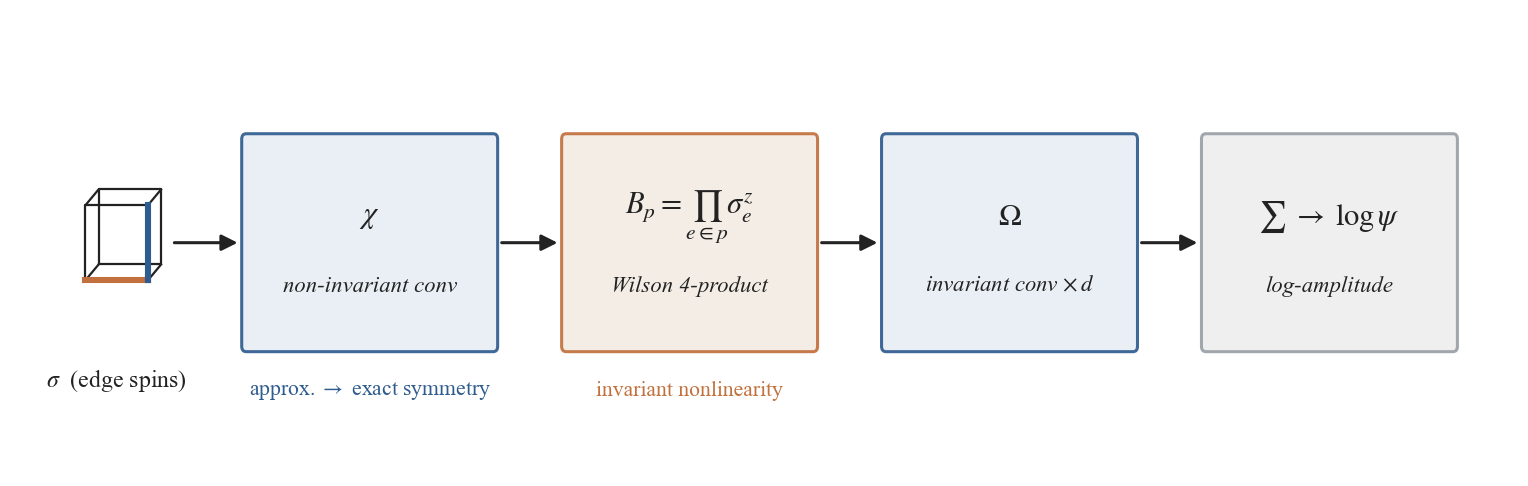
\includegraphics[width=\linewidth]{figures/arch_3d.png}
    \caption{The 3D combo architecture: edge spins $\sigma$ on the cubic lattice pass through the non-invariant convolution $\chi$, the invariant Wilson 4-product $B_p$, and the invariant convolution $\Omega$, before being summed into the log-amplitude.}
    \label{fig:arch3d}
\end{figure}

\subsection{Validation at $L=2$}
We first validated the architecture at $L=2$ with open boundary conditions, where exact diagonalization is still accessible, studying several variants by varying the network depth and width. Figure 4 shows that the symmetric combo architecture converges to the exact ground-state energy $E_0$ with a relative error of order $10^{-5}$, whereas an equivalent network without the built-in symmetry (a geometry-exact CNN with no Wilson product, translation-equivariant but not $A_v$-invariant) plateaus near $10^{-3}$. \textbf{The symmetry-free baseline gets trapped in a local optimum well above $E_0$, while the symmetric network reaches the exact energy to within its Monte-Carlo error.} This mirrors the 2D result and confirms that the built-in symmetry is what makes the ansatz both accurate and trainable at this scale.

\begin{figure}[H]
    \centering
    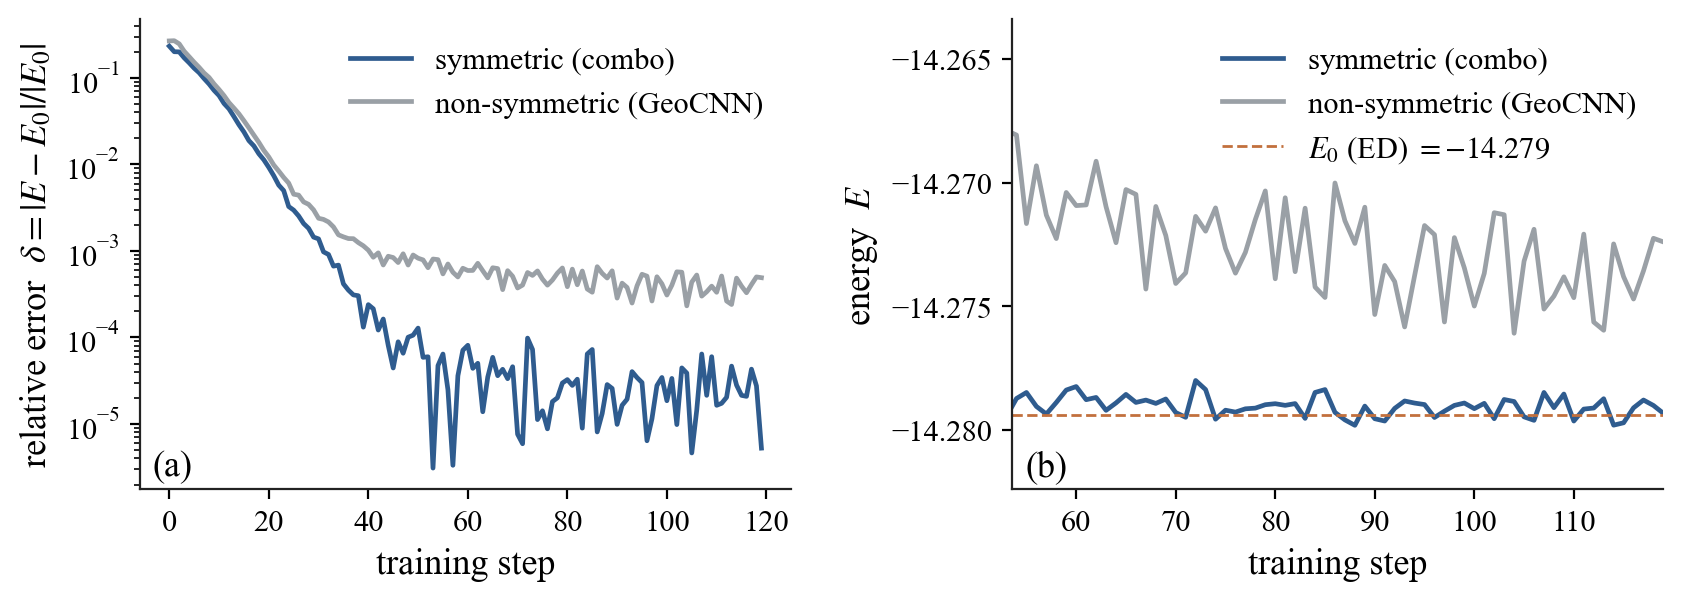
\includegraphics[width=\linewidth]{figures/validation_L2.png}
    \caption{Validation at $L=2$ (OBC) against exact diagonalization. (a) Relative energy error $\delta$ over training: the symmetric net reaches $\delta\sim10^{-5}$, the symmetry-free baseline plateaus near $10^{-3}$. (b) Energy near convergence; the symmetric net sits on the exact $E_0$ while the baseline remains visibly above it. Bands are the seed spread.}
    \label{fig:val}
\end{figure}

\subsection{Mapping the Phase Transition}
Having validated the architecture, we mapped the topological-to-trivial transition. We fixed $h_x=0.2$ and swept $h_z$, tracking the Fredenhagen--Marcu string order parameter $O_{FM}$ as a function of $h_z$ at $L=4,5,6$ ($L=7$ is not yet available). For each $L$ we fit $O_{FM}(h_z)$ to a sigmoid and located the transition $h_c(L)$ at the peak of its derivative (Figure 5a,b). A linear extrapolation of $h_c(L)$ in $1/L$ (Figure 5c) gives $h_c(\infty)\approx0.21$, \textbf{consistent with the Quantum Monte Carlo estimate $h_c\approx0.2$ for this model} and providing our first quantitative estimate of the 3D transition from NQS. The extrapolated value does depend on where the order-parameter string is placed: the bulk placement quoted above gives $h_c(\infty)\approx0.21$, whereas a boundary placement extrapolates higher, to $\approx0.34$ (Figure 5c, dashed).

\begin{figure}[H]
    \centering
    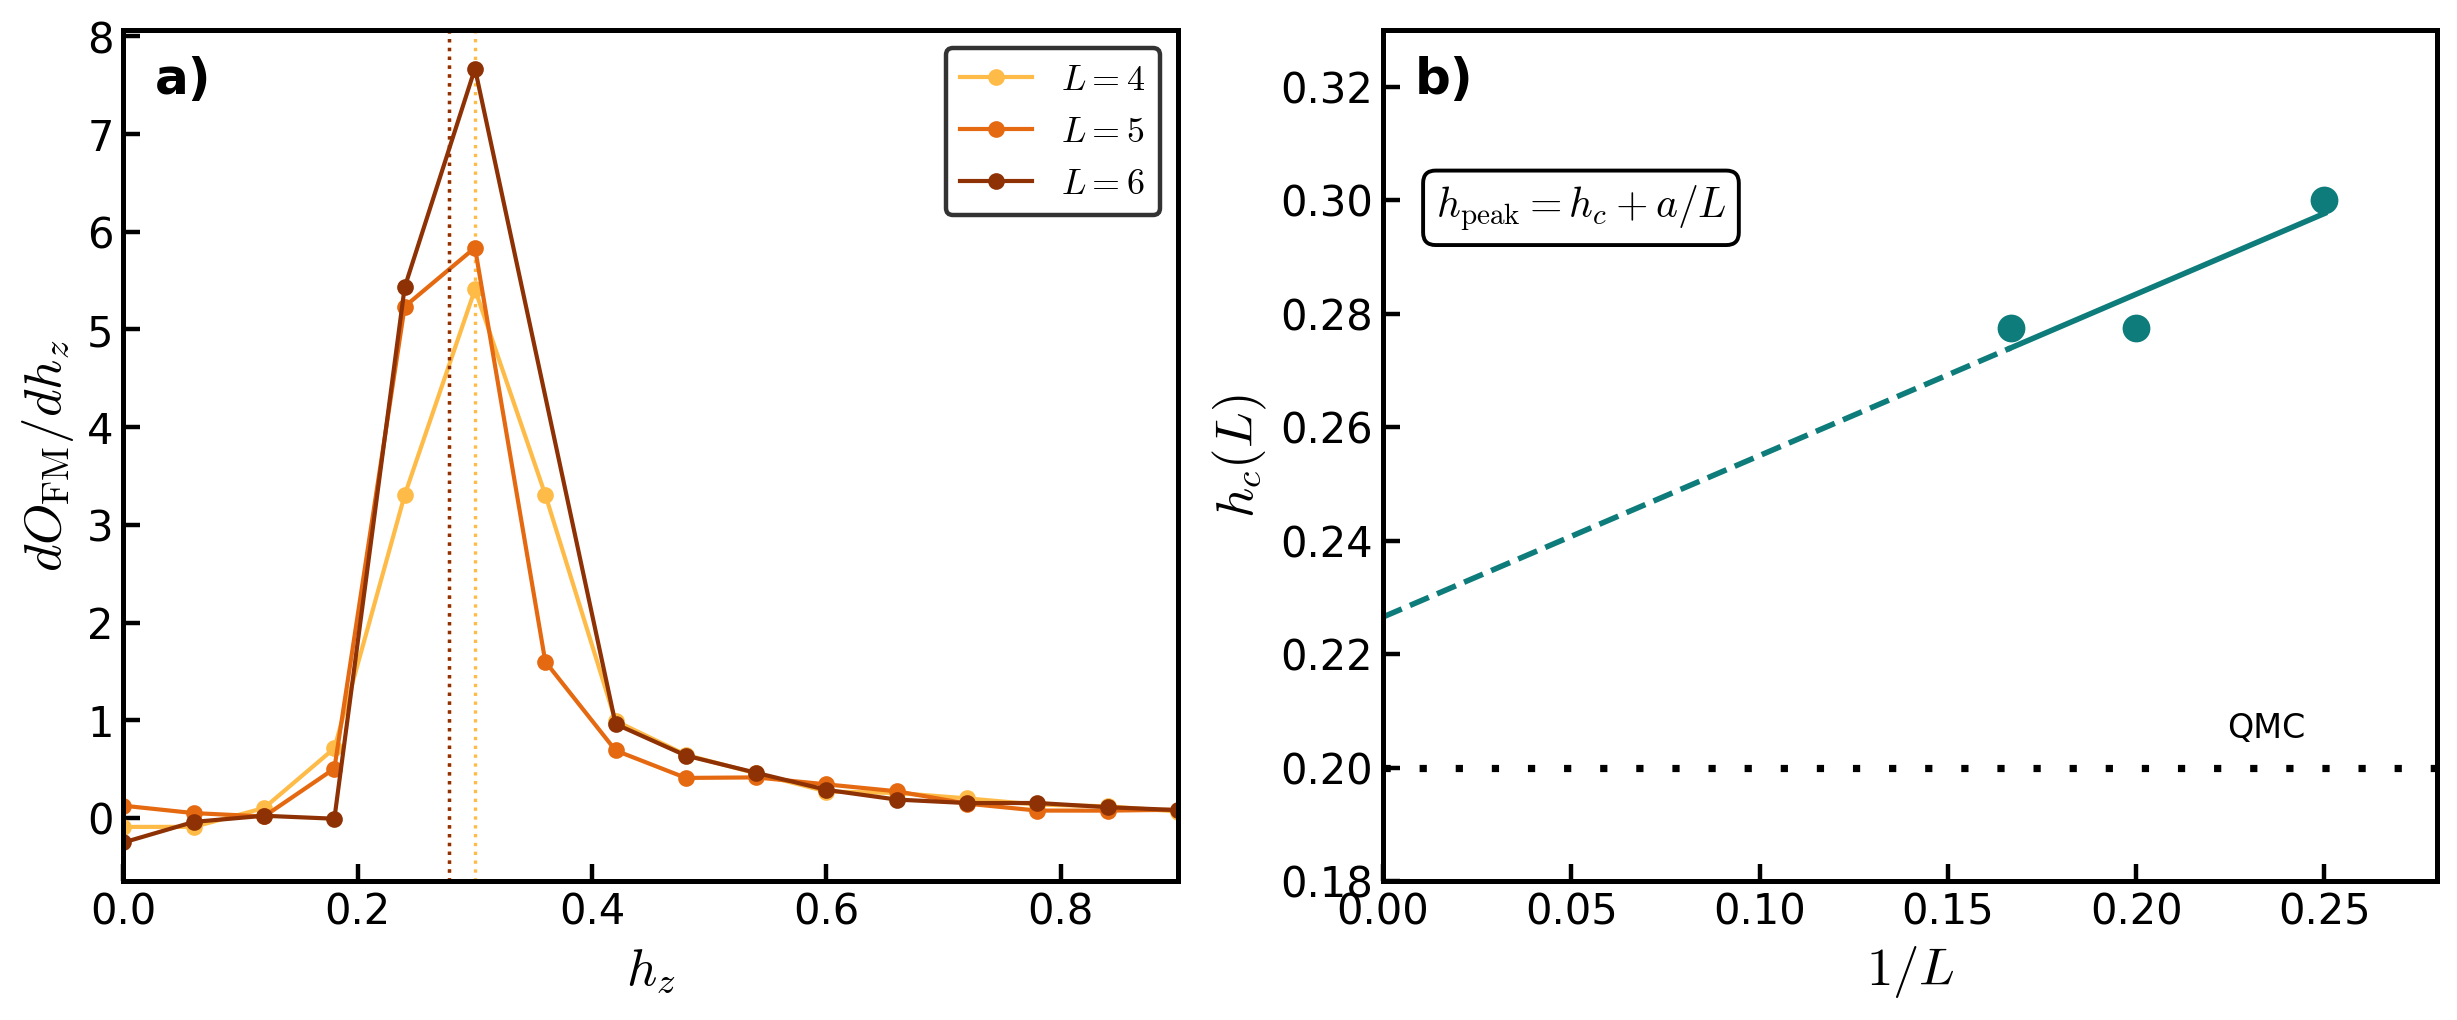
\includegraphics[width=\linewidth]{figures/transition.png}
    \caption{Topological$\to$trivial transition at $h_x=0.2$. (a) FM order parameter $O_{FM}(h_z)$ with sigmoid fits for $L=4,5,6$. (b) Its derivative, whose peak locates $h_c(L)$. (c) Finite-size extrapolation: the bulk placement gives $h_c(\infty)\approx0.21$ (solid); the boundary placement extrapolates higher (dashed).}
    \label{fig:trans}
\end{figure}

\paragraph{Methods.} All energies and order parameters are computed with variational Monte Carlo using stochastic reconfiguration, sampled with a Metropolis rule that combines single-spin flips with vertex-star cluster moves to remain within the topological sector. The Fredenhagen--Marcu order parameter $O_{FM}=\langle S\rangle/\sqrt{|\langle W\rangle|}$ is the ratio of an open Wilson string $S$ to the square root of the corresponding closed loop $W$, and distinguishes the deconfined (topological) phase from the trivial one.

\subsection{Limitations and Outlook}
The main limitation at present is the finite-size extrapolation, which rests on only three system sizes ($L=4,5,6$). We have already validated the architecture at $L=7$ (kernel size 5) and are currently mapping the $h_z$ transition line at that scale; a fourth data point should tighten the $1/L$ extrapolation and sharpen our estimate of $h_c$. We expect these results soon.



% \section{References}
% \begin{enumerate}
%     \item Preskill, J. (2000). Quantum information and physics: some future directions. Journal of Modern Optics, 47(2-3), 127-137.
%     \item Castelvecchi, D. (2017). Quantum computers ready to leap out of the lab in 2017. Nature, 541(7635), 9–10. https://doi.org/10.1038/541009a
% ‌    \item Huang, H.-L., Wu, D., Fan, D., & Zhu, X. (2020). Superconducting quantum computing: a review. Science China Information Sciences, 63(8). https://doi.org/10.1007/s11432-020-2881-9
%     \item Kitaev, A. Yu. (2003). Fault-tolerant quantum computation by anyons. Annals of Physics, 303(1), 2–30. https://doi.org/10.1016/S0003-4916(02)00018-0
% ‌    \item A Topologically Fault-Tolerant Quantum Computer with Four Dimensional Geometric Codes. (2025). Arxiv.org. https://arxiv.org/html/2506.15130v1#S4
%     \item Quintavalle, A. O., Vasmer, M., Roffe, J., & Campbell, E. T. (2021). Single-Shot Error Correction of Three-Dimensional Homological Product Codes. PRX Quantum, 2(2). https://doi.org/10.1103/prxquantum.2.020340
% ‌    \item Bañuls, M. C. (2023). Tensor Network Algorithms: A Route Map. Annual Review of Condensed Matter Physics, 14(1), 173–191. https://doi.org/10.1146/annurev-conmatphys-040721-022705
%     \item Kufel, D. S., Kemp, J., Vu, D., Linsel, S. M., Laumann, C. R., & Yao, N. Y. (2025). Approximately Symmetric Neural Networks for Quantum Spin Liquids. Physical Review Letters, 135(5), 056702–056702. https://doi.org/10.1103/pgnx-11ph
% ‌   \item Zhou, S.-T., Cheng, M., Rakovszky, T., von Keyserlingk, C., & Ellison, T. D. (2025). Finite-Temperature Quantum Topological Order in Three Dimensions. Physical Review Letters, 135(4). https://doi.org/10.1103/n9sq-8cxw
% \end{enumerate}
\pagebreak
\bibliographystyle{unsrt}
\bibliography{references}
\cite{preskill2000}
\cite{castelvecchi2017}
\cite{huang2020}
\cite{kitaev2003}
\cite{topological2025}
\cite{quintavalle2021}
\cite{banuls2023}
\cite{kufel2025}
\cite{zhou2025}
\end{document}


